\section{The algorithm} \label{sec:algorithm}

%%%%%%%%%%%%%%%%%%%%%%%%%%%%%%%%%%%%%%%%%%%%%%%%%%%%%%%%%%%%%%%%%%%%%%%%%%%%%%%%%%
%%%%%%%%%%  OVERVIEW
%%%%%%%%%%%%%%%%%%%%%%%%%%%%%%%%%%%%%%%%%%%%%%%%%%%%%%%%%%%%%%%%%%%%%%%%%%%%%%%%%%
\subsection{Overview} \label{sec:algorithm:overview}
The Omicron algorithm is developed in C++ and the code lives in the Virgo software repository~\cite{VirgoSVN}. Omicron is built upon GWOLLUM~\cite{GWOLLUM} libraries used to perform every step of an Omicron analysis. The GWOLLUM package depends on external libraries. The FrameL~\cite{FrameL} library is used to perform IO operations on data frame files~\footnote{The frame format was developed for interferometric gravitational-wave detectors' data.}. Mathematical routines developed in the GNU Scientific Library~\cite{GSL} are commonly used by GWOLLUM functions. Discrete Fourier transforms are performed using the FFTW~\cite{FFTW} algorithm. Finally, the GWOLLUM and Omicron codes heavily rely on C++ classes developed in the ROOT~\cite{Brun:1997pa} framework. For example, ROOT classes are used for plotting purposes, for event storage or for data access. To deal with package dependencies, the CMT~\cite{CMT} configuration management tool was chosen.

A fully object-oriented framework is adopted when developing GWOLLUM and Omicron, in which C++ classes and inheritance features are extensively used. The Omicron algorithm is entirely based on the \texttt{Omicron} C++ class which member functions are used to perform the analysis steps. A typical Omicron application can be represented by the sequence of functions represented in Fig.~\ref{fig:omicron_flowchart}. The \texttt{Omicron} constructor must be called using an input option file listing all the parameters defining the search one wants to perform. Then, the Omicron object must be provided with time segments to process. This is done with the \texttt{Omicron::InitSegment()} function. These time segments are processed sequentially with the \texttt{Omicron::NewChunk()} function. For every chunk, the list of channels to process is looped over with the \texttt{Omicron::NewChannel()} function. The input data vector is loaded with the \texttt{Omicron::LoadData()} function. The data is then conditioned; it is down-sampled to a working frequency and high-pass filtered. This is performed with the  \texttt{Omicron::Condition()} function. Before applying the $Q$-transform, the data is whitened by normalizing the data spectrum by the noise power spectrum density. The whitened data is finally projected onto a basis of windowed complex exponentials, as described in Sec.~\ref{sec:method}. This is done using the \texttt{Omicron::Project()} function. When calling the \texttt{Omicron::WriteOutput()} function, the Omicron data products are saved to disk\footnote{The html report is saved when calling the \texttt{Omicron} destructor.}.

\begin{figure}
  \center
  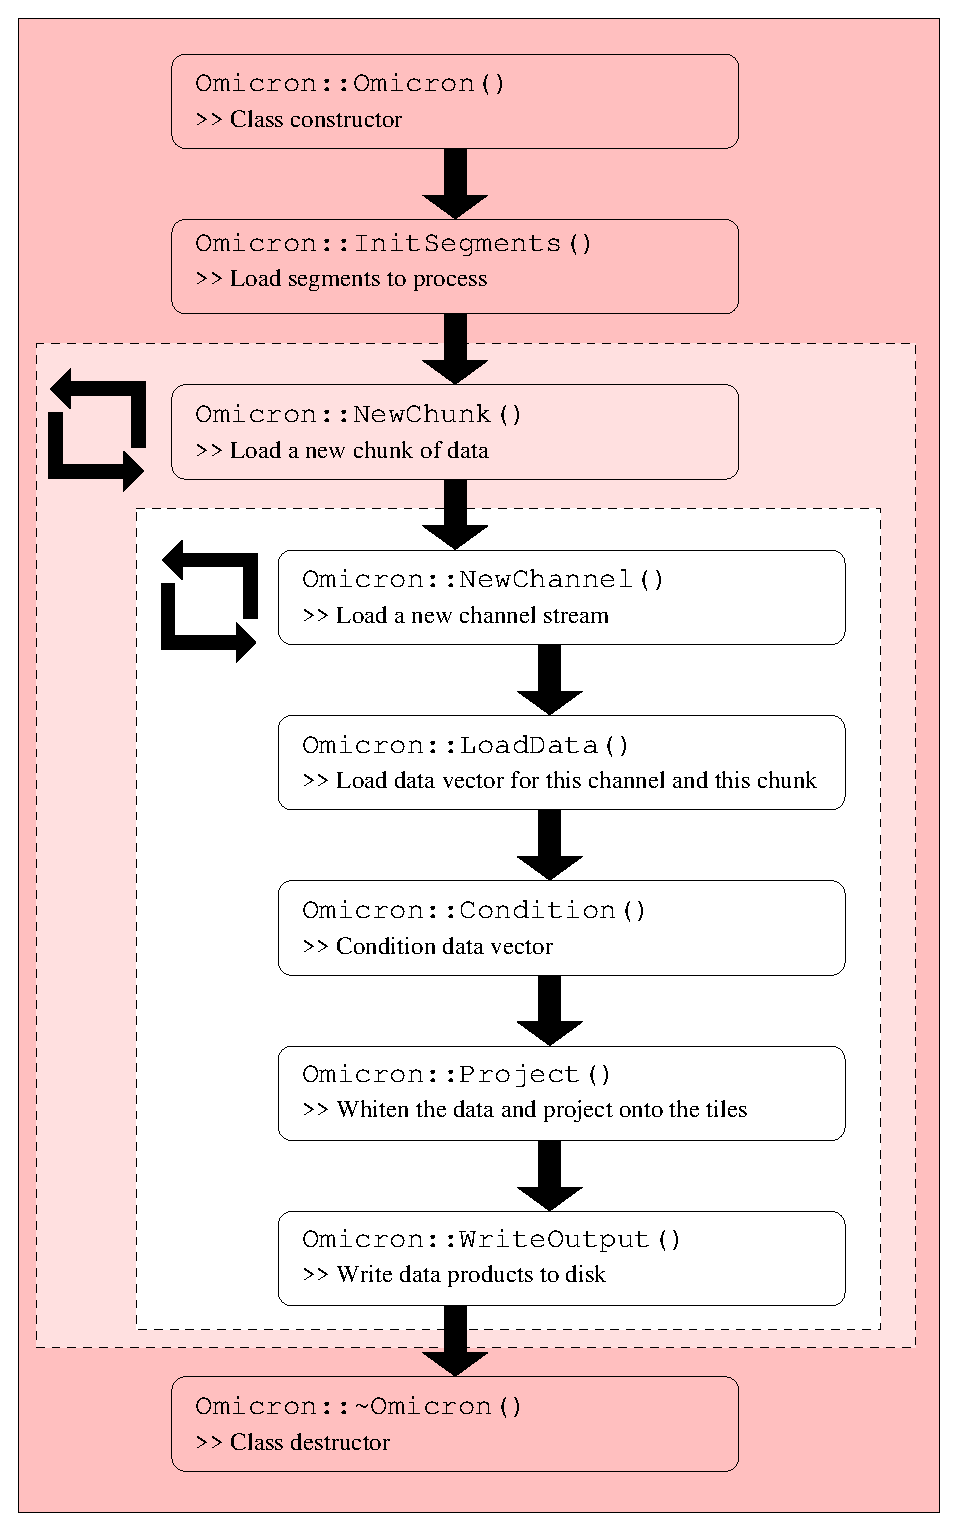
\epsfig{width=10cm, file=./figures/omicron_flowchart.eps}
  \caption{Standard \texttt{Omicron} analysis flowchart. The standard sequence of class functions is presented. Loops must be perfomed over data chunks and channels. They are represented by the dashed-line rectangles.}
  \label{fig:omicron_flowchart}
\end{figure}

This sequence of actions is performed by the \texttt{omicron.exe} executable. This programs runs the Omicron analysis using a list of arguments:
\begin{itemize}
  \item \texttt{omicron.exe gps\_start gps\_stop /path/to/parameters.file}. The Omicron algorithm is run over a single time segment starting at GPS time \texttt{gps\_start} and stopping at GPS time \texttt{gps\_end} and using the parameters listed in the file \texttt{/path/to/parameters.file}.
  \item \texttt{omicron.exe /path/to/segments.file /path/to/parameters.file}. The Omicron algorithm is run over all the time segments listed in \texttt{/path/to/segments.file} and using the parameters listed in the file \texttt{/path/to/parameters.file}.
  \item \texttt{omicron.exe gps\_center /path/to/parameters.file}. The Omicron algorithm is run over a single time chunk centered on GPS time \texttt{gps\_center} and using the parameters listed in the file \texttt{/path/to/parameters.file}.
\end{itemize}
The \texttt{Omicron} class offers more methods which can be used to tailor specfic applications. For an up-to-date and extensive description of these methods, refer to the doxygen documentation~\cite{Omicron_doxygen}.

%\begin{figure}
%  \center
%  \includegraphics[angle=90, scale=0.4]{./figures/omicron_incl}
%  \caption{Diagram presenting the Omicron code dependencies. Header files starting with a ``O'' are part of the Omicron Package. Header files starting with a ``T'' are taken from the ROOT~\cite{Brun:1997pa} libraries. \bluenote{Clean this!}}
%  \label{fig:omicron_incl}
%\end{figure}

%%%%%%%%%%%%%%%%%%%%%%%%%%%%%%%%%%%%%%%%%%%%%%%%%%%%%%%%%%%%%%%%%%%%%%%%%%%%%%%%%%
%%%%%%%%%%  DISCRETE
%%%%%%%%%%%%%%%%%%%%%%%%%%%%%%%%%%%%%%%%%%%%%%%%%%%%%%%%%%%%%%%%%%%%%%%%%%%%%%%%%%
\subsection{The discrete analysis} \label{sec:algorithm:discrete}

The Omicron algorithm is designed to process any data time series $x(t)$ associated to a gravitational-wave detector channel, e.g. the detector output channel, an environmental sensor, a photodiode signal, etc. The data consists of a discrete time sequence, $x[j]$, which is identified by a channel name and a native sampling frequency, $f_s$, defining the time separation between two consecutive data points $\delta t = t_{j+1}-t_j = 1/f_s$. As we will see in Sec.~\ref{sec:algorithm:conditioning}, the Omicron algorithm includes a data conditioning step where the input data is downsampled to a working sampling frequency $f_w$, allowing for an optimized subsequent processing. The data is then iteratively analyzed by time chunks of fixed duration $T_c$, corresponding to $N_c=T_cf_w$ data samples.

As presented in Sec.~\ref{sec:method}, the Omicron analysis requires to perform multiple Fourier transforms. The forward and inverse Fourier transforms of Eq.~\ref{eq:FTforward} and~\ref{eq:FTbackward} are discretized as 
\begin{equation}
  \tilde{x}[k]=\frac{1}{f_w}\sum_{j=0}^{N_c-1}{x[j]\mathrm{e}^{-2i\pi jk/N_c}}
\end{equation}
and
\begin{equation}
  x[j]=\frac{f_w}{N_c}\sum_{j=0}^{N_c-1}{\tilde{x}[k]\mathrm{e}^{+2i\pi jk/N_c}}.
\end{equation}
The frequency-domain data vector, $\tilde{x}$, is of size $N_c$ and the frequency sample interval is $\delta f = f_{k+1}-f_k = f_w/N_c = 1/T_c$. By convention, the first element, $\tilde{x}[0]$ is the DC component which is a purely real number. Positive frequencies are stored in the first half of $\tilde{x}$: $f_k=kf_w/N_c$, with $1\le k \le N_c/2$. The element $\tilde{x}[N_c/2]$ is purely real and is associated to the Nyquist frequency $f_{\text{Nyquist}}=f_w/2$. Negative frequencies are stored backward in the second half of $\tilde{x}$: $f_k=(k-N_c)f_w/N_c$, with $N_c/2 < k < N_c$.

Discrete Fourier transforms are performed with the FFTW~\cite{FFTW} algorithm. They can be computationally expensive and care must be taken to optimize the use of FFTW routines.

A first approach is to only work with vector sizes which are a power of two. In this configuration, the FFTW routines provide optimal performance. With Omicron, the working sampling frequency $f_w$ and the chunk duration $T_c$ are required to each be a power of two. Therefore $N_c$ is a power of two.

Another possibility of optimization is to take advantage from the fact that, most often, we work with purely real data vectors. For instance, the detector signal $x[j]$ is a purely real time series. As a result, the spectrum, $\tilde{x}[k]$, is symmetrical around DC. The negative frequencies are ignored and only one-sided data vectors are considered: $\tilde{x}$ is of size $N_c/2+1$. This redundancy is expoited by the FFTW algorithm to reduce the computing cost, both memory and speed.



%%%%%%%%%%%%%%%%%%%%%%%%%%%%%%%%%%%%%%%%%%%%%%%%%%%%%%%%%%%%%%%%%%%%%%%%%%%%%%%%%%
%%%%%%%%%%  TILING
%%%%%%%%%%%%%%%%%%%%%%%%%%%%%%%%%%%%%%%%%%%%%%%%%%%%%%%%%%%%%%%%%%%%%%%%%%%%%%%%%%
\subsection{Tiling the parameter space} \label{sec:algorithm:tiling}

When the \texttt{Omicron} constructor is called, the tiling structure described in Sec.~\ref{sec:method:tiles} is created using the parameters listed in the user option file. The targeted parameter space must be specified: the $Q$ range, $[Q_{min}; Q_{max}]$, the frequency range, $[\phi_{min}; \phi_{max}]$ and a time range. The time range is fixed to the characteristic chunk duration, $T_c$, and is centered on 0: $[-T_c/2; +T_c/2]$. If necessary, the $Q_{min}$ and $\phi_{max}$ parameters are automatically adjusted so that they verify the anti-aliasing conditions~\ref{eq:antialias1} and~\ref{eq:antialias2}. In addition, in order to get a reasonable noise estimate \bluenote{(reference)}, it is required to work with an integrated mismatch distance along the time dimension $s_\tau\ge50$, which translates into a minimum permissible frequency, $\phi_{min} \ge 50Q/(2\pi T_c)$.
The user options must also include the maximum fractional energy loss due mismatch, $\mu_{max}$, from which the number of tiles used to cover the parameter space is determined.

A $Q$ plane object is implemented as a C++ class inheriting from the 2-D histogram class of ROOT (\texttt{TH2D}). The number of $Q$ planes, $N_Q$, is equal to the next integer verifying condition~\ref{eq:tiledistanceq}. The $Q$ planes, indexed by $q$, are given a $Q$ value obtained from Eq.~\ref{eq:q}.

A $Q$ plane histogram is then vertically binned into logarithmically-spaced frequency rows. The number of frequency rows, $N_\phi(Q_q)$, is equal to the next integer verifying condition~\ref{eq:tiledistancephi}. For each frequency row $(q,l)$, the horizontal time axis is divided into $N_\tau(Q_q,\phi_l)$ linear bins, $N_\tau(Q_q,\phi_l)$ being the next power of two verifying the condition~\ref{eq:tiledistancetau}. Indeed, in Sec.~\ref{sec:algorithm:discrete}, we explained that working with power-of-two vector sizes is computationally more efficient. The tile time and frequency, $(\tau_{q,lm,} \phi_{q,l})$, is given by the histogram bin center obtained from~Eq.\ref{eq:tau} and~\ref{eq:phi}. It also useful to give the histogram bin width in both the time and frequency dimensions:
\begin{align}
  \Delta\tau_{q,l,m} &= T_c / N_\tau(Q_q, \phi_{q,l}), \label{eq:dtau} \\
  \Delta\phi_{q,l} &= 4\phi_{l}\sqrt{\frac{\mu_{max}}{3(2+Q_l^2)}}.\label{eq:dphi}
\end{align}


A realistic example of a tiling structure is represented in Fig.~\ref{fig:tiling}, using the parameters listed in Appx~\ref{appx:parameters}. With this setting, 5 $Q$ planes are generated, representing a total of 2,098,688 tiles over a chunk of $T_c=64$~s and between $\phi_{min}=40.0$~Hz and $\phi_{max}=489.2$~Hz. For the plane with the lowest-$Q$ value, the time resolution varies between 0.98~ms and 7.81~ms and the frequency resolution spans from 8.9~Hz to 54.5~Hz. For the highest-$Q$ plane, the time resolution varies between 7.81~ms and 125.00~ms and the frequency resolution spans from 8.9~Hz to 54.5~Hz.
\begin{figure}
  \center
  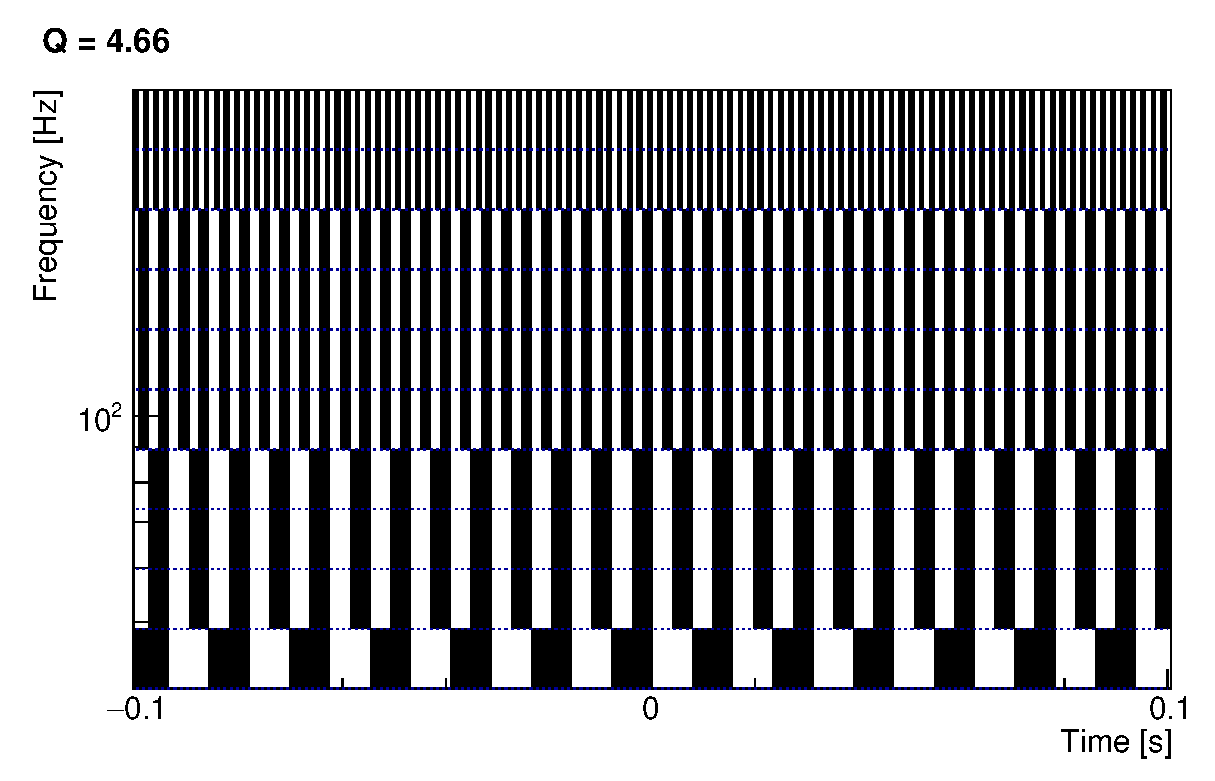
\epsfig{width=7.5cm, file=./figures/q0.eps} 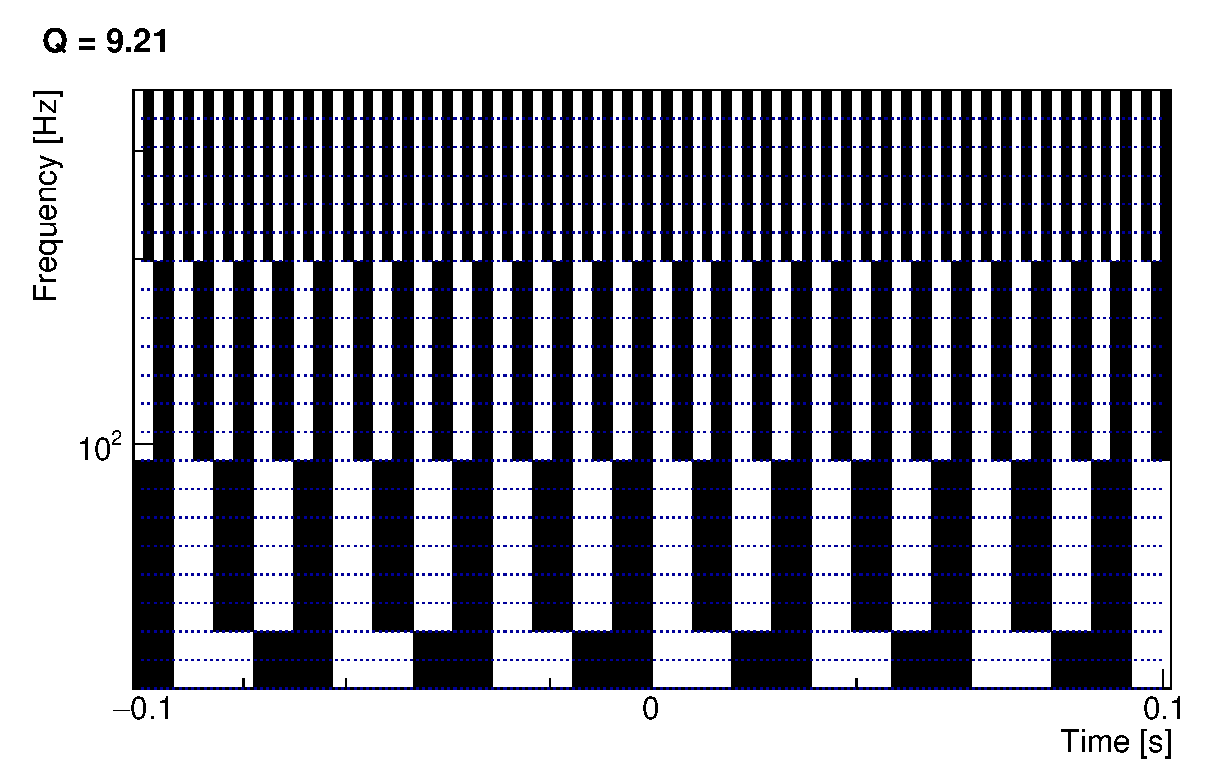
\epsfig{width=7.5cm, file=./figures/q1.eps} \\
  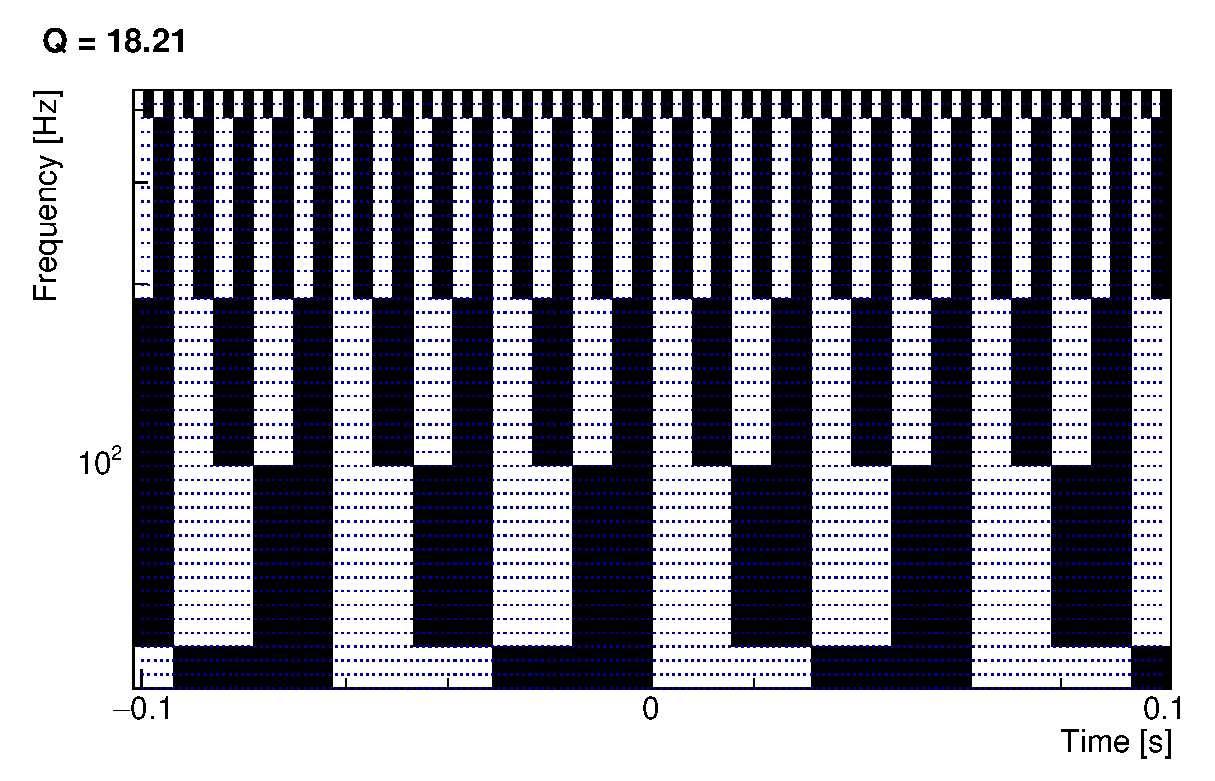
\epsfig{width=7.5cm, file=./figures/q2.eps} 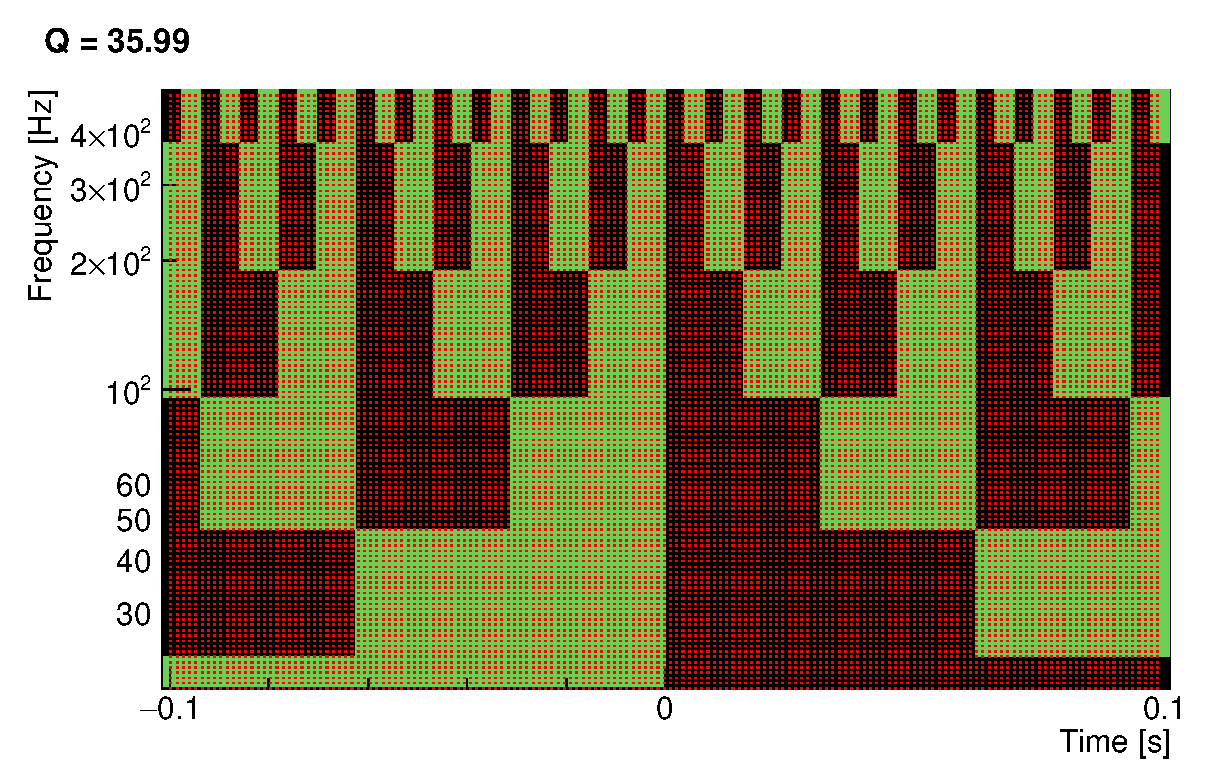
\epsfig{width=7.5cm, file=./figures/q3.eps} \\
  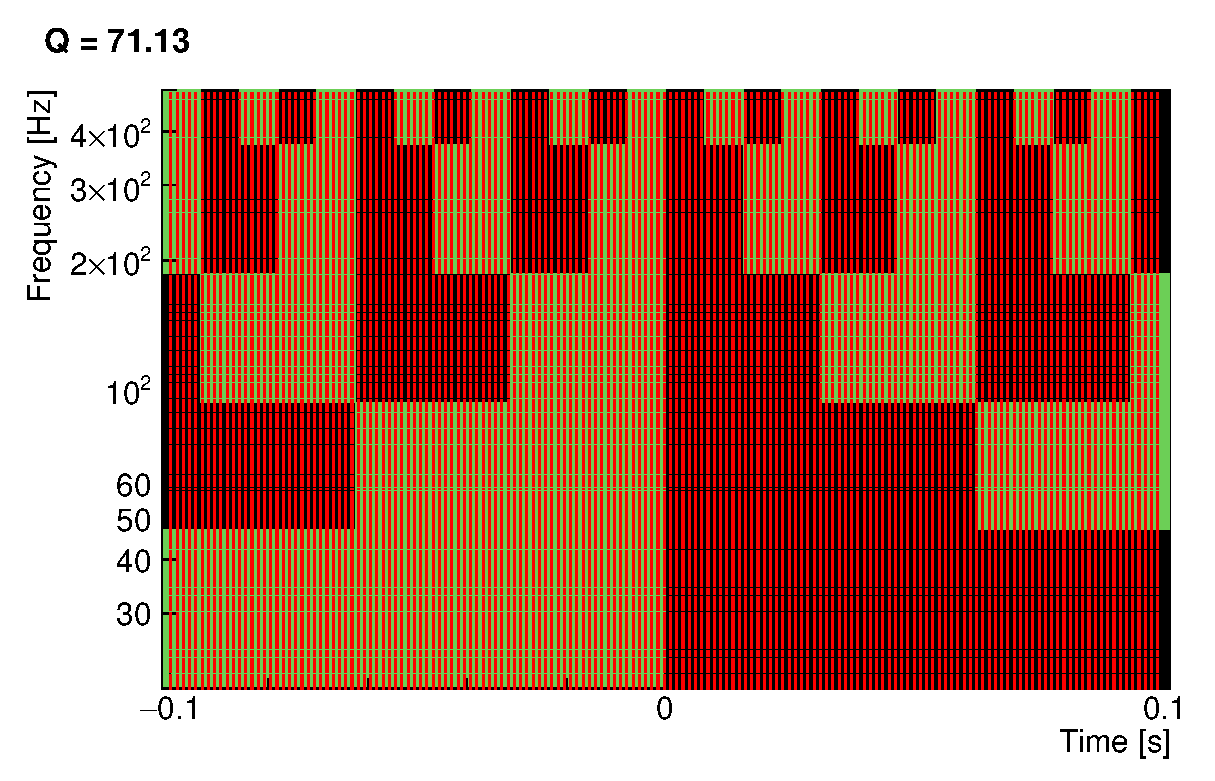
\epsfig{width=7.5cm, file=./figures/q4.eps}
  \caption{Example of a realistic tiling structure using the parameters given in Appx~\ref{appx:parameters}. When requiring a maximal energy loss of $\mu_{max}=20\%$, 5 $Q$ planes are needed to cover the $Q$ range $[\sqrt{11}; 100]$. Each $Q$ plane is then tiled (black and white rectangles) along frequency rows delimited by the blue dashed lines. To distinguish the tiles, the time chunk is zoomed in $\pm 100$~ms.}
  \label{fig:tiling}
\end{figure}

%%%%%%%%%%%%%%%%%%%%%%%%%%%%%%%%%%%%%%%%%%%%%%%%%%%%%%%%%%%%%%%%%%%%%%%%%%%%%%%%%%
%%%%%%%%%%  Windows
%%%%%%%%%%%%%%%%%%%%%%%%%%%%%%%%%%%%%%%%%%%%%%%%%%%%%%%%%%%%%%%%%%%%%%%%%%%%%%%%%%
\subsection{The windows} \label{sec:algorithm:window}
As presented in Eq.~\ref{eq:qtransform2}, the $Q$ transform includes windowing the data in the frequency domain. In Sec.\ref{sec:method:window}, we discussed the possibility of using a bisquare window to approximate the ideal Gaussian window. Such a bisquare window is generated for each frequency row $l$ of each $Q$ plane $q$ composing the tiling structure presented in Sec.~\ref{sec:algorithm:tiling}. The window expression, given in Eq.~\ref{eq:bisquare}, must be discretized using the conventions defined in Sec.~\ref{sec:algorithm:discrete}:
\begin{equation}
  \tilde{w}_{ql}[k] =
  \begin{cases}
    W_b \left[1 - \left(\frac{2k}{M_{ql}-1}\right)^2 \right]^2 & 0\le k \le \frac{M_{ql}-1}{2}, \\
    W_b \left[1 - \left(\frac{2(k-N_c)}{M_{ql}-1}\right)^2 \right]^2 & N_c-\frac{M_{ql}-1}{2}\le k < N_c, \\
    0 & \textrm{otherwise},
  \end{cases}
  \label{eq:dbisquare1}
\end{equation}
where $M_{ql}=2\lfloor \delta f(\phi_{q,l},Q_q) T_c \rfloor + 1$ is the window size, obtained using the relation $\delta f(\phi_{q,l},Q_q) = \phi_{q,l}\sqrt{11}/Q_q$.


%Before performing the analysis of Eq.~\ref{eq:qtransform3}, the data vector $x$ is whitened such that individual samples of the resulting discrete time sequence are statistically independent random variables with zero mean and unit variance.


%%%%%%%%%%%%%%%%%%%%%%%%%%%%%%%%%%%%%%%%%%%%%%%%%%%%%%%%%%%%%%%%%%%%%%%%%%%%%%%%%%
%%%%%%%%%%  DATA ACCESS
%%%%%%%%%%%%%%%%%%%%%%%%%%%%%%%%%%%%%%%%%%%%%%%%%%%%%%%%%%%%%%%%%%%%%%%%%%%%%%%%%%
\subsection{The data access} \label{sec:algorithm:data}
The input data time series is read using the FrameL~\cite{FrameL} library, developed to perform read/write file operations using the Frame format\footnote{The frame format is a data format specifically developed for interferometric gravitational-wave detectors.}. The data must be provided through a Frame File List (FFL) file which consists in an ASCII file with the file extension ``.ffl''. This file must contain a list of frame files described over five columns: the path to the frame file, the GPS information for the file start, the file duration in seconds, the GPS time of the first event and the GPS time of the last event\footnote{A FFL file can be obtained using the FrameL program \texttt{FrDump.exe}: \texttt{FrDump.exe -i /path/to/frame/files/*.gwf -d 0 $>$ fflfile.ffl}}. The GWOLLUM class, \texttt{ffl}, is designed to offer an improved C++ interface to access frame data. For example, the \texttt{ffl} class provides compatibility with the specific LIGO lal-cache file format.

The \texttt{ffl} class is used by Omicron to load data by time chunks. The chunk is an important charactistic time scale which is user-defined in the parameter file. It defines the time sequence adopted to analyze the data. The chunk duration, $T_c$, directly determines the size of Omicron data containers: $N_c=f_wT_c$.

Fig.~\ref{fig:segmentation} presents how the input data is segmented and analyzed. The input time segments, provided by the Omicron command line, are subdivided into chunks. The size of the chunks is fixed and is defined in the user parameter file. Chunks overlap by a fixed amount of time. The overlap duration, $T_o$, is also defined in the user parameter file. The segment size does not generally matches the chunk and overlap structure. As a result, for the last chunk, the overlap is adjusted to fit the current segment size. The overlapping structure is introduced to manage edge artifacts due to the forward and backward filtering of the data (see Sec.~\ref{sec:algorithm:conditioning}). Some data is irremediably lost in this process: segments shorter than the chunk duration cannot be analyzed and the first and last edges of a segment (half the overlap) are not saved.
\begin{figure}
  \center
  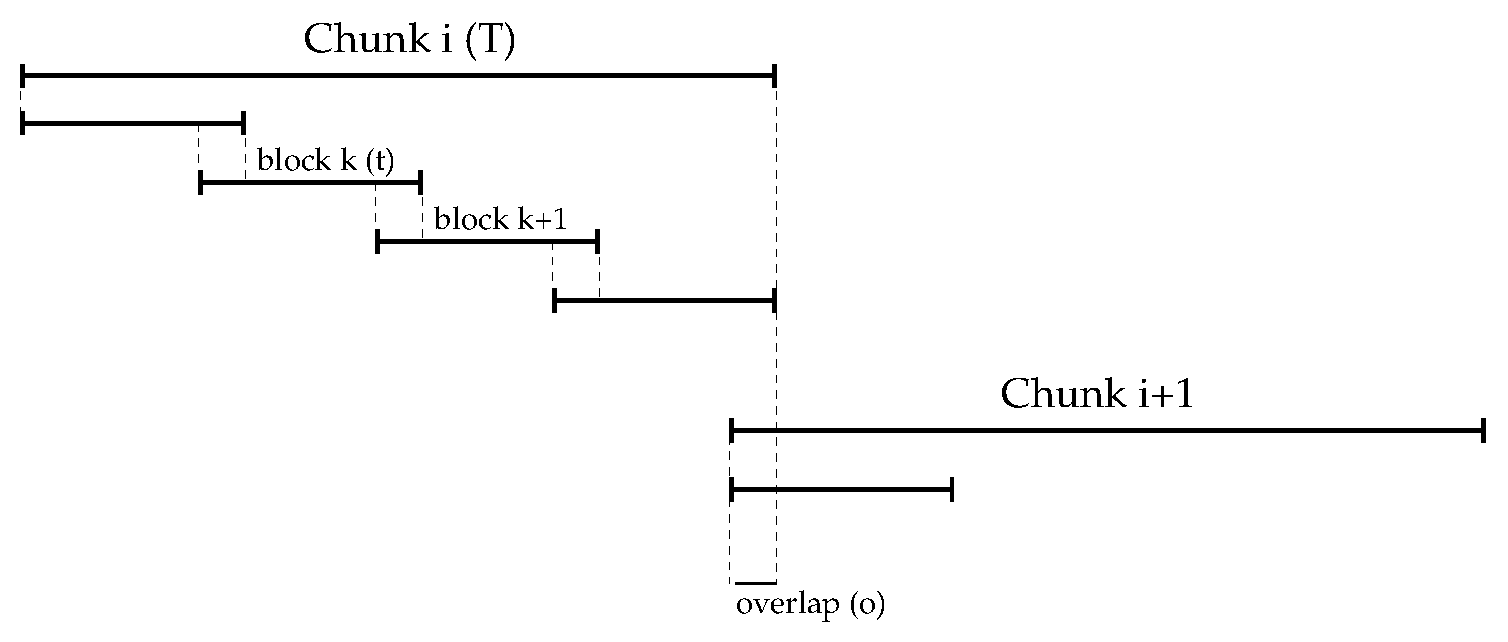
\epsfig{width=15cm, file=./figures/segmentation.eps}
  \caption{Data segmentation. The input segments are analyzed sequentially, chunk by chunk. The chunks, represented by the red lines, have a fixed size and are defined in the user parameter file. They overlap by a fixed amount of time, also defined in the parameter file. The overlap for the last chunk of a segment is modified to adjust the segment size. Only the central part of the chunk, represented by the black lines, is meaningful. Only Omicron triggers in this central region are saved.}
  \label{fig:segmentation}
\end{figure}

The chunk and overlap structure must verify some conditions:
\begin{enumerate}
\item The durations must be integer values. Omicron only supports integer durations.
\item The chunk duration must be a power of 2 value and longer than or equal to 4 seconds.
\item The overlap duration must be an even value and shorter than the chunk duration for obvious reasons.
\end{enumerate}

Chunks and channels are internally looped over using the \texttt{Omicron::NewChunk()} and \texttt{Omicron::NewChannel()} functions. For a given chunk and a given channel, a data vector is filled with the raw time series, using the \texttt{Omicron::LoadData()} function. The native sampling frequency for the channel data stream, $f_s$, is directly determined by the size of the vector which is loaded. This is checked for every chunk. This way, a change of the channel native sampling frequency is automatically accounted for when looping over the chunks.


%%%%%%%%%%%%%%%%%%%%%%%%%%%%%%%%%%%%%%%%%%%%%%%%%%%%%%%%%%%%%%%%%%%%%%%%%%%%%%%%%%
%%%%%%%%%%  DATA CONDITIONING
%%%%%%%%%%%%%%%%%%%%%%%%%%%%%%%%%%%%%%%%%%%%%%%%%%%%%%%%%%%%%%%%%%%%%%%%%%%%%%%%%%
\subsection{The data conditioning} \label{sec:algorithm:conditioning}
The chunk data vector is transformed to optimize the performance of the subsequent processing. It is downsampled to a lower working frequency, $f_w$, to maximize the processing speed and lower the memory usage. It is then high-pass filtered to reduce the signal dynamic range. The filtering C++ code is inspired from the routines developed in the LSC Algorithm Library Suite~\cite{LALSUITE}.

To avoid aliasing, a 20$^{\mathrm{th}}$-order Butterworth low-pass filter with an attenuation factor of 0.1 is applied using a cutoff frequency set at the targeted Nyquist frequency, $f_w/2$. The filter is applied in the time domain first forwards and then backwards in order to cancel the phase delay introduced by a single pass. The disadvantage of the Butterworth filter is that, since it is an IIR filter, it is not possible to determine the exact length of corrupted data at the start and end of the output time series. The chunk overlap duration (see Sec.~\ref{sec:algorithm:data}) must be chosen with care to reject these filtering artifacts. Finally, the time-series is decimated to the desired working sampling frequency. The resulting working data vector size is now reduced to $N_c=f_w \times T_c$.

The working vector is high-pass filtered using a 12$^{\mathrm{th}}$-order Butterworth filter. This is done with zero phase distortion by first forward filtering and then reverse filtering the working vector. Once again, the chunk overlap duration must be long enough to remove the filtering artifacts. The filter frequency cutoff is determined by the lower end of the search frequency range, $\phi_{min}$, defined by the user in the parameter file.

The conditioning of the data is illustrated in Fig.~\ref{fig:conditioning}. Omicron is run using the parameter file given in Appx.~\ref{appx:parameters}. The input data is originally sampled at 16384~Hz, the spectrum of which is represented in black in the upper plot. First, it is downsampled at a working frequency of 1024~Hz. The resulting spectrum is represented in blue and ends at the Nyquist frequency of 512~Hz. After the high-pass filter, frequencies below 40~Hz are attenuated as shown by the red spectrum. The ratio of spectra of the different filtering steps are plotted in the middle and at the bottom of Fig.~\ref{fig:conditioning}.
\begin{figure}
  \center
  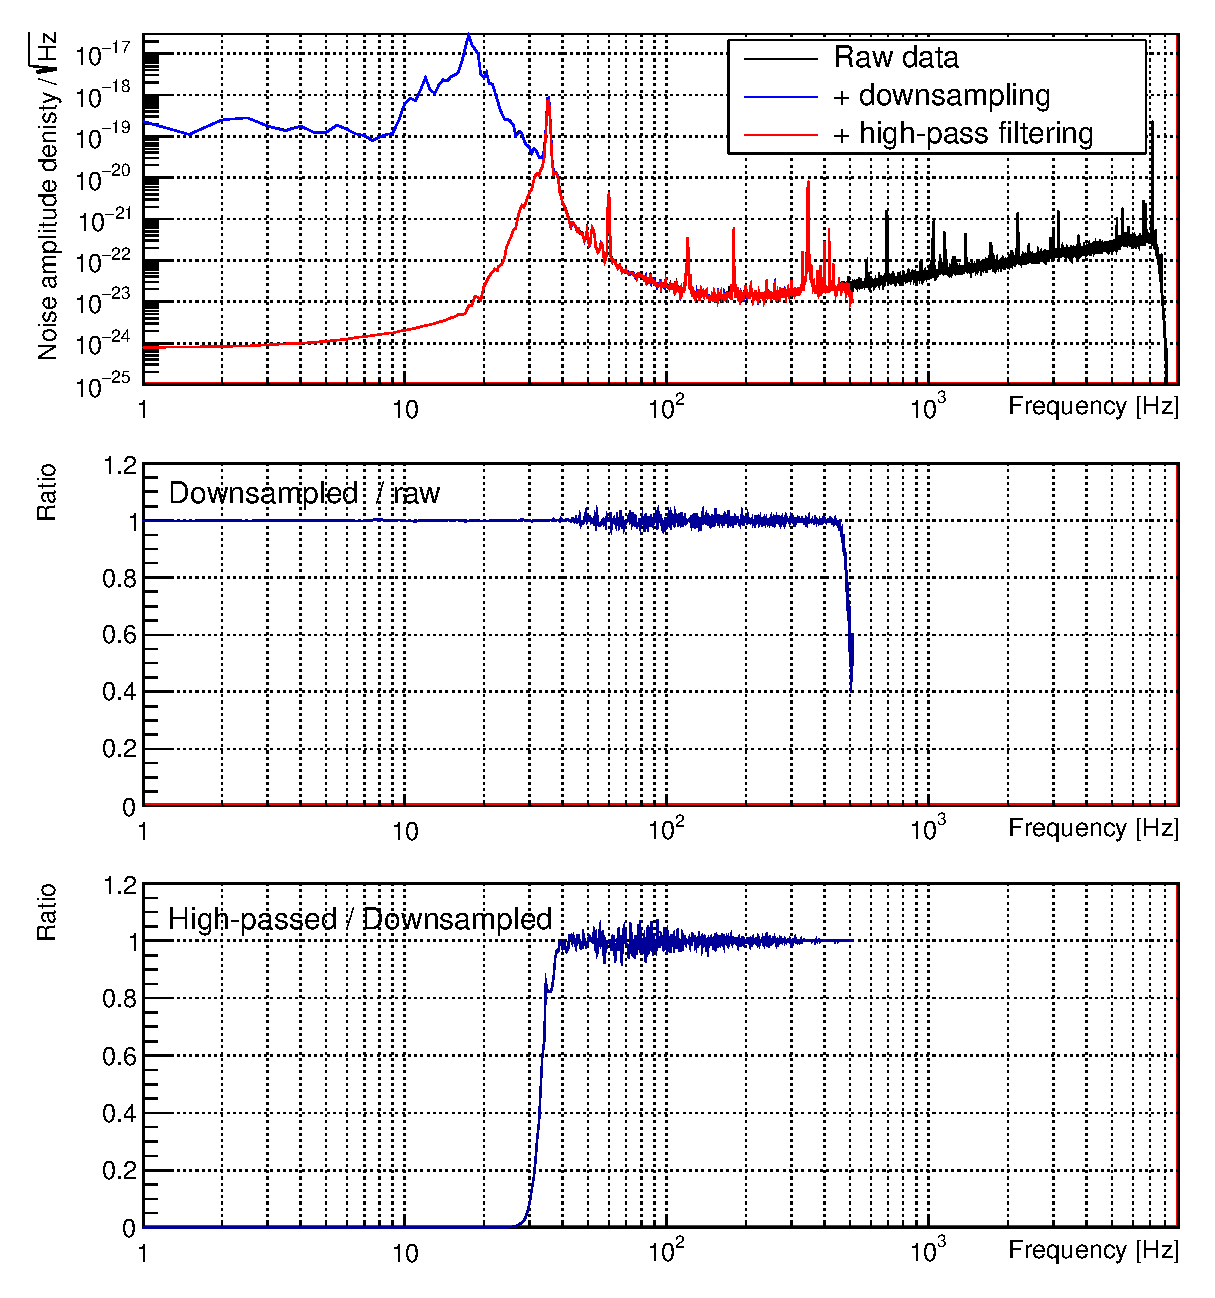
\epsfig{width=10cm, file=./figures/conditioning.eps}
  \caption{The upper plot displays the noise data spectra measured at different steps of the conditioning process. The black curve presents the spectrum of the raw data between 1~Hz and the Nyquist frequency of 8192~Hz. The raw data are downsampled to a working frequency $f_w=1024$~Hz. The resulting spectrum is represented in blue. The downsampled data is then high-pass filtered ($f>40$~Hz) and the measured spectrum is represented in red. The ratio between the downsampled and the raw spectrum is plotted in the middle. The lower plot shows the ratio between the high-passed and the downsampled spectra.}
  \label{fig:conditioning}
\end{figure}

The final step of the conditioning process consist of applying a Tukey window to the time-series, offering a smooth transition to 0 at both chunk ends. The expression of the Tukey window implemented in \texttt{Omicron} is:
\begin{equation}
  w_{\mathrm{tukey}}(t) = 
  \begin{cases}
     \frac{1}{2}\left[ 1+\cos{\left(2\pi\frac{t}{T_o}-\pi\right)}\right]& t < T_o/2, \\
     \frac{1}{2}\left[ 1+\cos{\left(2\pi\frac{(t-T_c)}{T_o}+\pi\right)}\right]& t > T_c-T_o/2, \\
     1.0 & \mathrm{otherwise}.
  \end{cases}
\end{equation}
Fig.~\ref{fig:tukey} presents examples of Tukey windows using several overlap durations.
\begin{figure}
  \center
  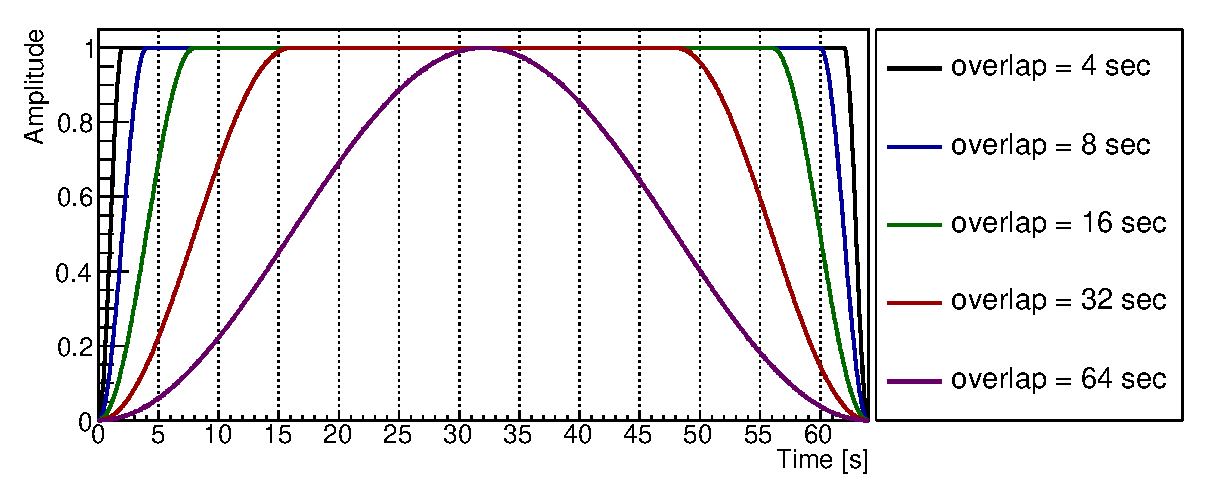
\epsfig{width=10cm, file=./figures/tukey.eps}
  \caption{Tukey windows used to smoothly transition the data time series to 0. A cosine function is applied at both chunk ends over half the overlap duration. Here, we used $T_c=64$~s and $T_o = 4$, 8, 16 and 32 s.}
  \label{fig:tukey}
\end{figure}

The data conditioning is performed using the \texttt{Condition()} function of the \texttt{Omicron} class. Before leaving this function, the data power spectrum density is updated using the newly conditioned data vector. This is described in the next section. 


%%%%%%%%%%%%%%%%%%%%%%%%%%%%%%%%%%%%%%%%%%%%%%%%%%%%%%%%%%%%%%%%%%%%%%%%%%%%%%%%%%
%%%%%%%%%%  DATA WHITENING
%%%%%%%%%%%%%%%%%%%%%%%%%%%%%%%%%%%%%%%%%%%%%%%%%%%%%%%%%%%%%%%%%%%%%%%%%%%%%%%%%%
\subsection{The data whitening} \label{sec:algorithm:whitening}

As described in Sec.~\ref{sec:method:whitening}, the $Q$ transform is applied over whitened data. The conditioned chunk data vector elements are re-weighted using the power spectral density. The PSD is estimated using the method developed for the \texttt{FINDCHIRP} algorithm~\cite{Allen:2005fk}. This method, inspired from the Welch method~\cite{Welch:1967}, offers a reliable and robust PSD estimate for non-Gaussian data.

A time-domain data vector $d$ of duration $T_\mathrm{PSD}$ and sampled at the Omicron working frequency $f_w$ is divided into sub-vectors $d_s$. The corresponding sub-segments of duration $T_\mathrm{spec}$, are indexed by $s$ and overlap by 50\%, as represented at the top of Fig.~\ref{fig:psdseg}. The one-sided periodograms are computed for all sub-segments using $f_wT_\mathrm{spec}$ data points and a normalized\footnote{the window is normalized such that $\sum_{j=0}^{f_wT_\mathrm{spec}-1}{w_H^2[i]} = f_wT_\mathrm{spec}$} Hann window, $w_H$:
\begin{align}
  P_s[k] &= \frac{2}{T_\mathrm{spec}}\left|\widetilde{(w_Hd_s)}[k]\right|^2 \\
  &= \frac{2}{T_\mathrm{spec}f_w^2}\left|\sum_{j=0}^{f_wT_\mathrm{spec}-1}{d_s[j]w_H[j]e^{-2i\pi jk/(f_wT_{spec})}}\right|^2.
\end{align}

To work with independent random quantities, the sub-segments are separated into two sets of non-overlapping segments: $N^e$ sub-segments with even indexes and $N^o$ sub-segments with odd indexes. Instead of using a mean, as prescribed with the Welch method, we use a median which offers a more robust estimator for the power spectrum. However, as explained in \cite{Allen:2005fk}, the resulting median value must be corrected by a bias factor $\alpha(N)=\sum_{n=0}^{N-1}{(-1)^{n+1}/n}$: $S^e[k]=\mathrm{median}(P_0[k], P_2[k],...)/\alpha(N^e)$ and $S^o[k]=\mathrm{median}(P_1[k], P_3[k],...)/\alpha(N^o)$. The final PSD is obtained by taking the mean of even and odd PSDs: $S[k]=(N^eS^e[k]+N^oS^o[k])/(N^e+N^o)$.
\begin{figure}
  \center
  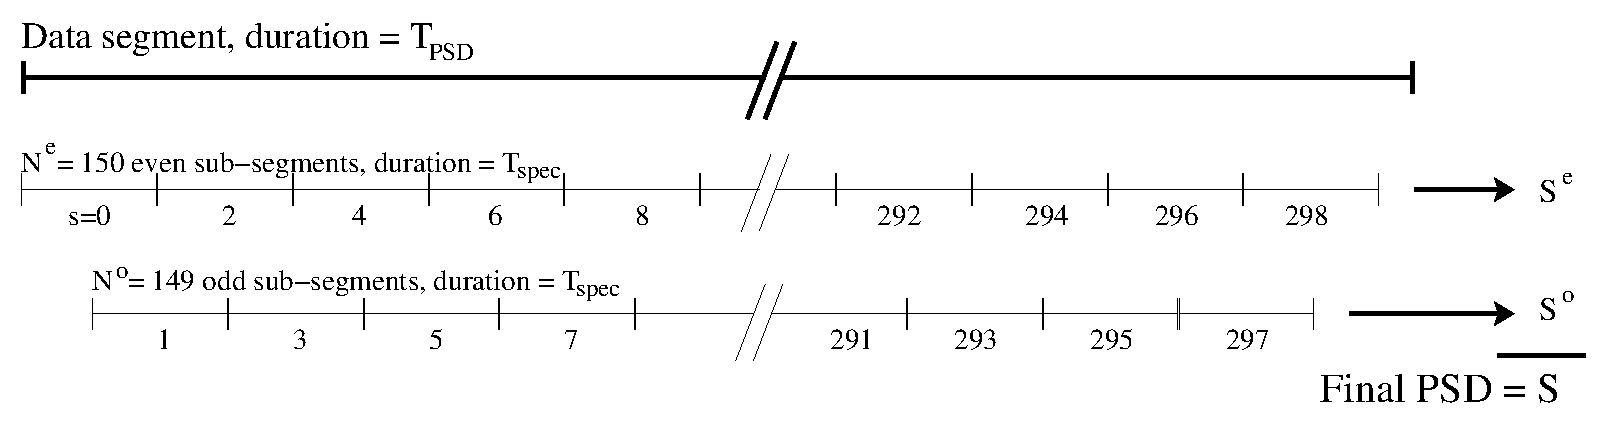
\epsfig{width=15cm, file=./figures/psdseg.eps} \\
  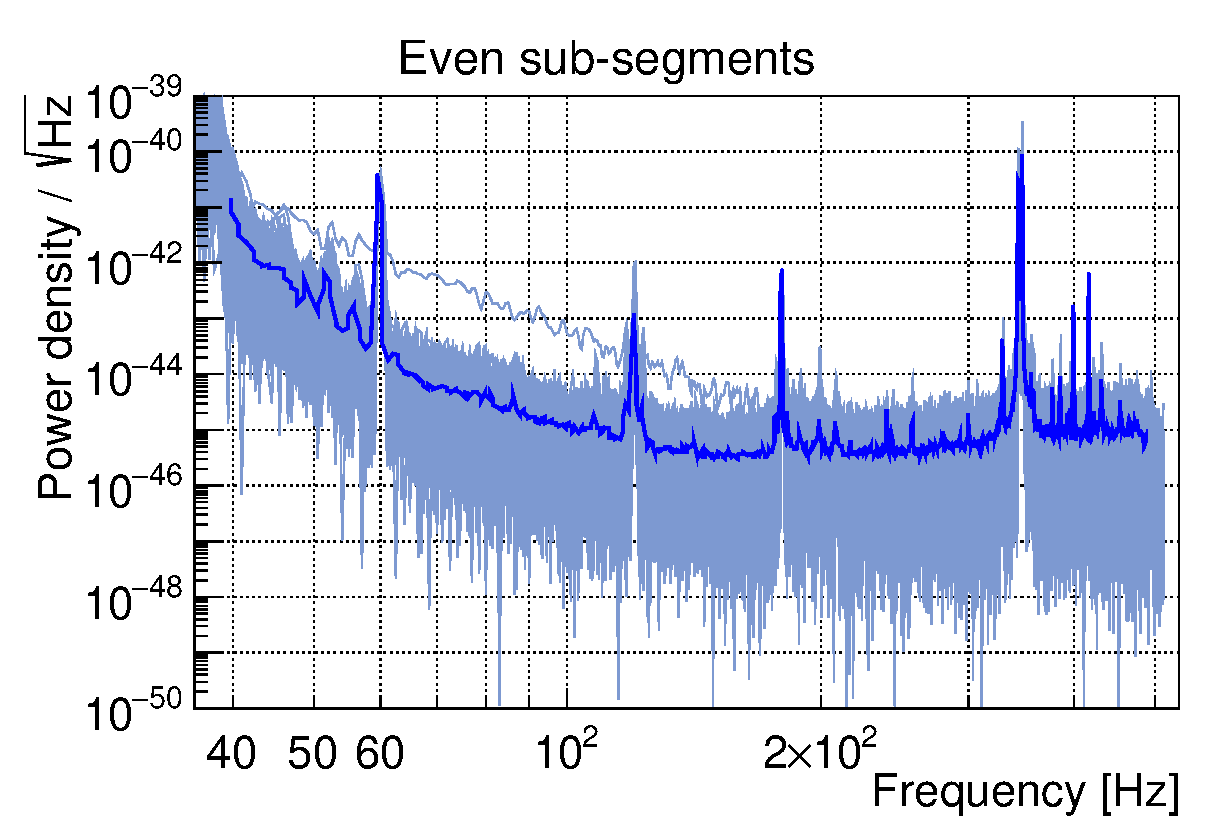
\epsfig{width=8cm, file=./figures/psd_even.eps}
  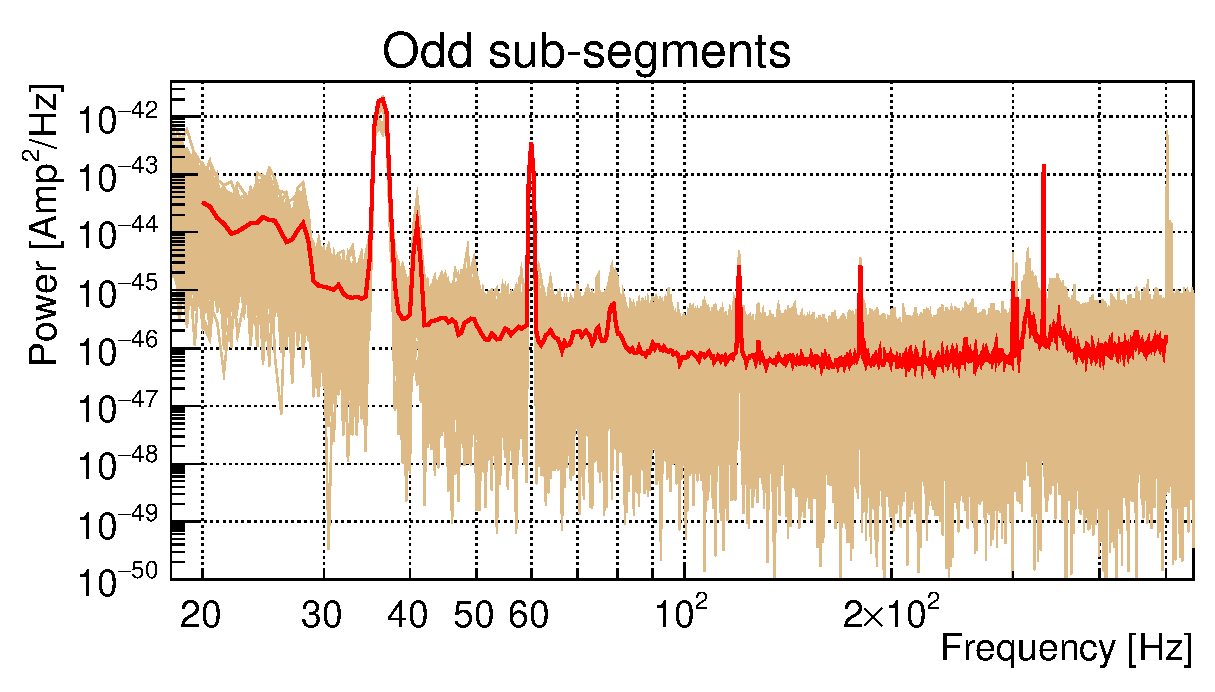
\epsfig{width=8cm, file=./figures/psd_odd.eps}
  \caption{The top panel presents the data segmentation used to estimate the noise power spectral density. The data segment of duration $T_\mathrm{PSD}$ is divided into two sets of non-overlapping sub-segments of duration $T_\mathrm{spec}$: the ``odd'' and ``even'' sets. The odd sub-segments are shifted by $T_\mathrm{spec}/2$ with respect to the even sub-segments. Note that a small time segment at the end of the data segment is left unused. The power spectral density is estimated for even sub-segments (bottom-left panel) and for odd subsegments (bottom-right pannel). The individual periodograms are displayed with dimmed lines while the resulting median PSD is plotted with a thick line. The odd and even PSDs are averaged into the final PSD. This example was obtained using the Omicron configuration given in Appx.~\ref{appx:parameters}: 150 even subsegments and 149 odd sub-segments were used to cover an input data vector of duration $T_\mathrm{PSD}=300$~s.}
  \label{fig:psdseg}
\end{figure}

For Omicron, the time scale to estimate the PSD is decoupled from the chunk structure; $T_\mathrm{PSD}$ can be set independently from the $T_c$ parameter, using the option file. When a new data chunk is loaded, the data vector, excluding half the overlap on both chunk edges, is saved in a circular buffer of duration $T_\mathrm{PSD}$. For each chunk, the PSD is then estimated using the data available in the buffer. If $T_\mathrm{PSD} > T_c-T_o$, the PSD is not optimally estimated for the first chunks as the circular buffer is not full. Using $T_\mathrm{PSD} < T_c-T_o$ is equivalent to a situation where $T_\mathrm{PSD} = T_c-T_o$. The PSD circular buffer is flushed whenever a new time segment starts (the time segments are described in Sec.~\ref{sec:algorithm:data}). 

The PSD frequency resolution must be compatible with the Omicron tiling structure described in Sec.~\ref{sec:algorithm:tiling} and be high enough to resolve all the $Q$ plane frequency rows. It is set by the hard-coded parameter $T_\mathrm{spec}$. If the search frequency range, $[\phi_{min}; \phi_{max}]$, is above 1~Hz, $T_\mathrm{spec}=2$~s. The PSD frequency resolution is then fixed at $1/T_\mathrm{spec}=0.5$~Hz. If the search frequency range goes below 1~Hz, $T_\mathrm{spec}=\lceil4/\phi_{min}\rceil$.

Before projecting the data onto the tiling structure, the data chunk, $x$, is Fourier-transformed and whitened as presented in Eq.~\ref{eq:white}. However, the PSD, $S$, and the data vector, $\tilde{x}$, do not have the same frequency resolution; by construction, the PSD resolution is lower than the data resolution.  To re-weight the data data sample $\tilde{x}[k]$, a linear interpolation is used to estimate the PSD value at the frequency $k/T_c$. Fig.~\ref{fig:white} illustrates the effect of the whitening method on the power spectral density. \bluenote{comment figure.}
\begin{figure}
  \center
  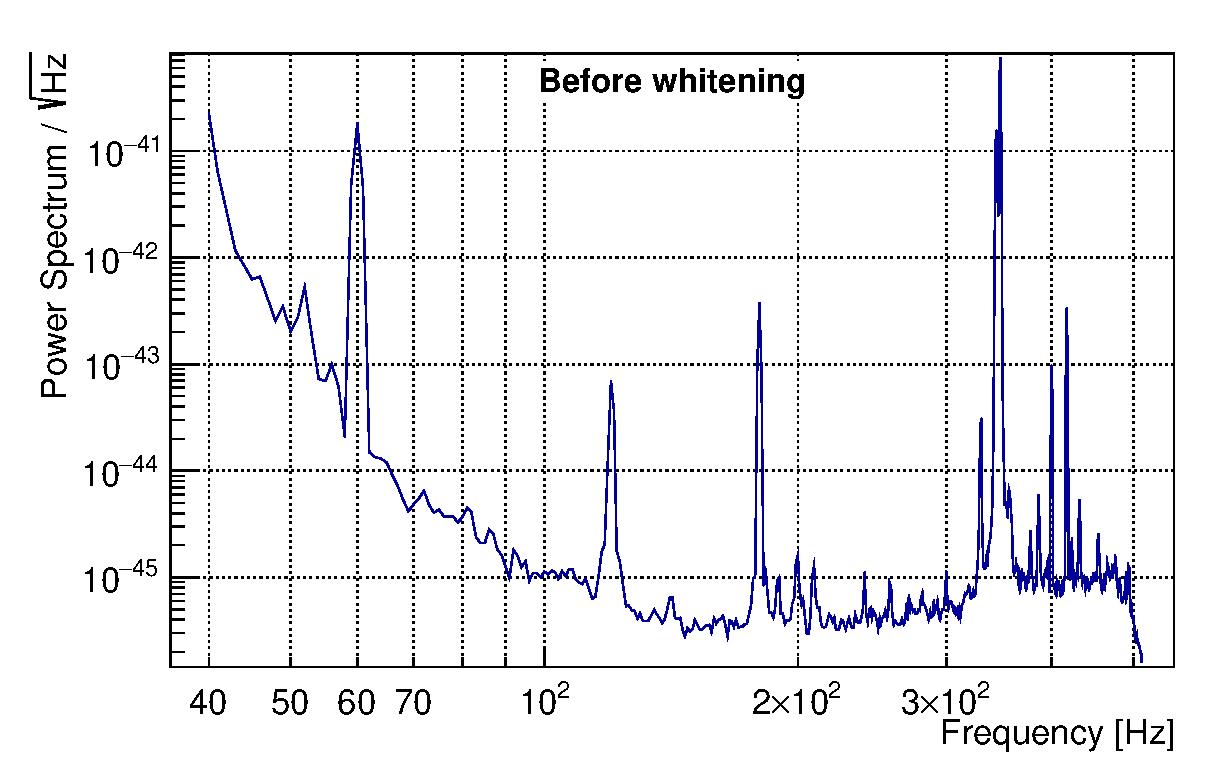
\epsfig{width=10cm, file=./figures/white_1.eps} \\
  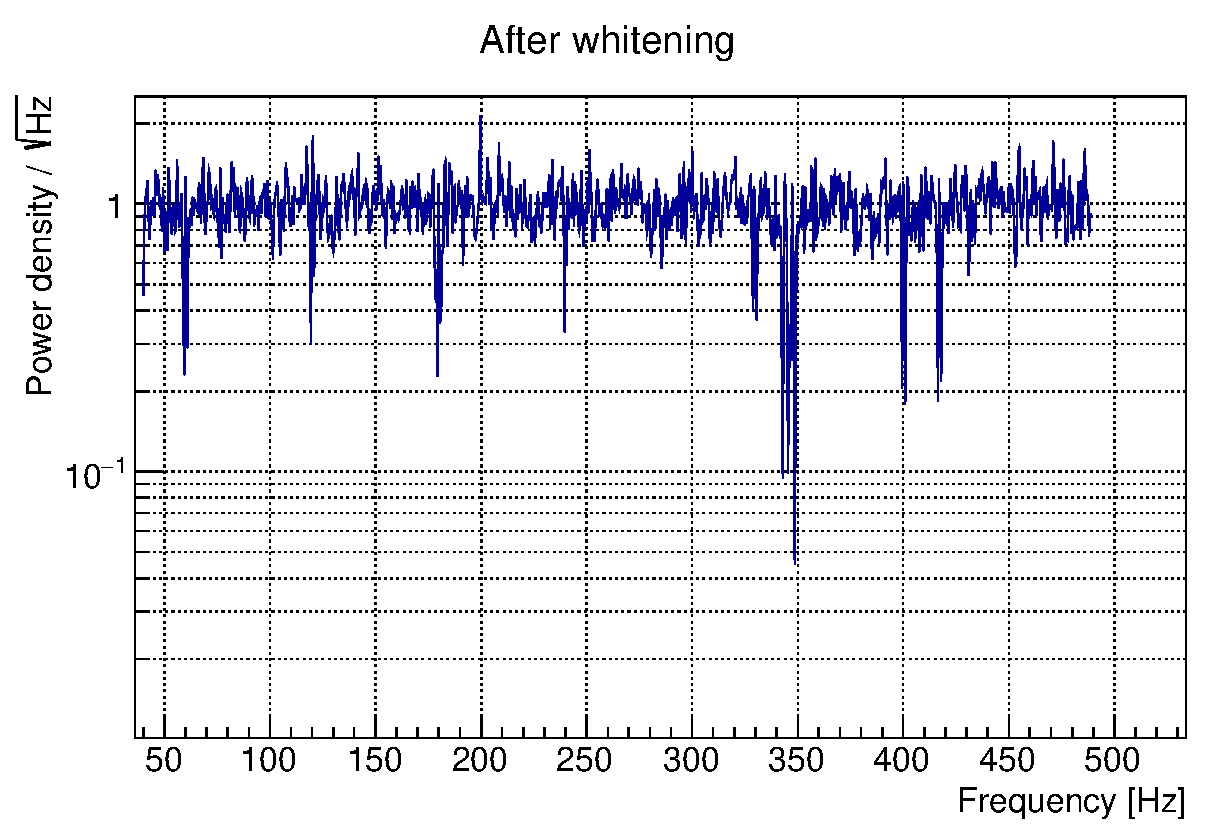
\epsfig{width=10cm, file=./figures/white_2.eps}
  \caption{Power spectral density before (top) and after (bottom) whitening the input data chunk.}
  \label{fig:white}
\end{figure}

%%%%%%%%%%%%%%%%%%%%%%%%%%%%%%%%%%%%%%%%%%%%%%%%%%%%%%%%%%%%%%%%%%%%%%%%%%%%%%%%%%
%%%%%%%%%%  DATA PROJECTION
%%%%%%%%%%%%%%%%%%%%%%%%%%%%%%%%%%%%%%%%%%%%%%%%%%%%%%%%%%%%%%%%%%%%%%%%%%%%%%%%%%
\subsection{The data projection} \label{sec:algorithm:projection}

The whitened frequency-domain data vector $\tilde{x}$ must be applied the $Q$ transform of Eq.~\ref{eq:qtransform2} for each tile $(m, l, q)$.

%As suggested in Sec.~\ref{sec:method:window}, in order to optimize the algorithm performance, the inverse Fourier transform of Eq.~\ref{eq:qtransform3} is performed over a reduced vector size. The window takes non-zero values between $\pm \Delta f$; the number of data points to consider is therefore $M=2\lfloor \Delta f(\phi_l,Q_q) T_c \rfloor + 1$.


\subsection{The triggering} \label{sec:algorithm:triggering}

\subsection{The mapping} \label{sec:algorithm:mapping}
